\documentclass[]{article}
\usepackage[ngerman]{babel}
\usepackage{natbib}
\usepackage{graphicx}
\usepackage[utf8]{inputenc}

%opening
\title{Abschlussbericht Semantic Argument Classification}
\author{Julian Baumann, Kevin Decker, Maximilian Müller-Eberstein}


\begin{document}

\maketitle

\section{Einleitung}
Unter Semantic Argument Classification versteht man, einem Satz seine semantische Rollen wie zum Beispiel Subjekt, Prädikat und Objekt zuzuweisen. Vereinfacht gesagt versucht man zu klären, "wer wem was antut". Sie gehört zum grundlegenden Pre-Processing für verschiedene Natural Language Processing-Anwendungen wie zum Beispiel Machine Translation und ist aus diesem Grunde auch ein wichtiger Aspekt der Forschung. Angelehnt an die Veröffentlichung von \cite{Pradhan05supportvector} versuchten wir im Verlauf unseres Projekts diese Aufgabe automatisch und überwacht durch Machine Learning-Ansätze umzusetzen. 

\section{Grundlagen}
\subsection{Daten und Tools}
Als Grundlage für unsere Experimente wurden verschiedene Datensätze und Tools verwendet. Wichtigste Ressourcen waren dabei PropBank und PennTree Bank. PropBank \cite{Palmer:2005:PBA:1122624.1122628} oder auch Proposition Bank ist ein Korpus in dem für jedes in ihm enthaltene Verb annotiert wurde, welche semantische Rollen es besetzt. Dies ist in Form von sogenannten Frames organisiert, welche auf mehr oder weniger lesbare Weise kodieren, welche Argumente überhaupt gefordert werden können. Im Gegensatz zu FrameNet, welches das gleiche versucht, ist PropBank jedoch nicht ganz so spezifisch sondern versucht durch generellere Argumente für möglichst viele Parser verwendbar zu sein.\\ 

\begin{table}
	\centering
	\begin{tabular}{|c|l|}
	\hline 
	ARG0 & proto-agent \\ 
	\hline 
	ARG1 & proto-patient \\ 
	\hline 
	ARG2 & instrument, benefactive, attribute \\ 
	\hline 
	ARG3 & starting point, benefactive, attribute \\ 
	\hline 
	ARG4 & ending point \\ 
	\hline 
	ARGM & modifier \\ 
	\hline 
	\end{tabular}
	\caption{Argumente der PropBank}
	\end{table}
	Die PennTree Bank \cite{Marcus93buildinga} ist ein Subkorpus des Wall Street Journals(WSJ) bestehend aus etwa einer Millionen Tokens. Davon sind etwa 112.917 Prädikat-Argument Strukuren nach dem PropBank-Schema annotiert. 
	\\
	Die oben genannten Korpora bilden die Grundlage für die im Folgenden näher erklärten Experimente.
	Zur Extraktion der Features wurde die Programmiersprache Python in der Version 3.4 zusammen mit dem Natural Language Toolkit \(Version 3.0\) verwendet. Die eigentliche Anwendung der Machine-Learning Algorithmen wurde in Weka \cite{Hall+FHPRW:2009} realisiert.
	\\
	Zur Klassifikation sollten drei verschieden Algorithmen verwendet werden:
	Der Naïve Bayes und der J48-Algorithmus, sowie eine Support
	Vector Machine. Letztere wurde ausgewählt, um den Experimentausgang mit den Ergebnissen von \cite{Pradhan05supportvector} zu vergleichen, die ebenfalls eine Support Vector Machine verwenden.
	Wie später im Abschnitt Experimente genauer beschrieben wird, lieferte der Naïve Bayes die zuverlässigsten Ergebnisse. 
	
	



%Datenvorstellung, Tools, Algorithmen
%Vergleichsgrundlagen
\section{Umsetzung} 

%umsetzung
\section{Features}
\subsection{einzelne Features}
Für das Experiment wurden 5 Features extrahiert und ihr Einfluss auf die Ergebnisse getestet. Das erste Feature, \textbf{Predicate}, ist einfach die lemmatisierte Form des Prädikats. In unserem Datenset trat dieses Feature in 3966 verschiedenen Werten auf. Zweites Feature, \textbf{Path}, beschreibt den Weg, der in einem Syntaxbaum durchlaufen werden muss, um vom Prädikat des Satzes zum Argument in Frage zu gelangen. Dies wird durch $\uparrow$ und $\downarrow$ gekennzeichnet. Dieses Feature hat sehr viele verschiedene Ausprägungen( 41737 distinct values), die durch verschiedene Satzstrukuren verursacht werden. 

\centering	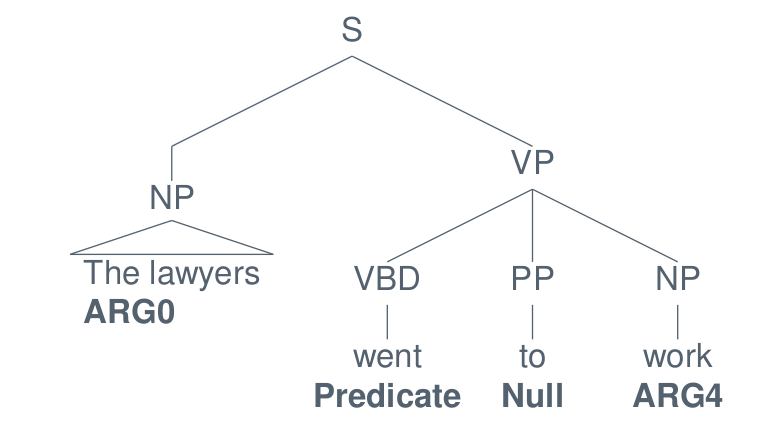
\includegraphics[scale=0.4]{Syntaxbaum}


Im Satz \glqq The lawyers went to work\grqq\ würde dieses Feature beispielsweise den Wert 
$ NP\uparrow S\downarrow VP\downarrow VBD$ annehmen. Im Feature \textbf{Phrase Type} ist kodiert, welcher Wortart(also NP, VP, etc.) das gesuchte Argument angehört. In unserem Fall sind dies 65 verschiedene Kategorien. 
Die anderen beiden Features \textbf{Position} und \textbf{Voice} sollten beide intuitiv betrachtet binär sein, durch die unvollständige Annotation in Propbank ist dies im Falle von Voice, also ob das Argument passiv oder aktiv ist, nicht der Fall. Hier gibt es noch einen dritten Wert unknown, wenn für das Prädikat keine Angabe diesbezüglich gemacht wurde. Position hingegen ist ein rein binäres Feature und gibt an, ob das Argument vor oder nach dem Prädikat auftritt. 

\subsection{Featureextraktion}

\section{Experimente}
\subsection{Probleme}

\section{Evaluation}
\subsection{Probleme}

\section{Retrospektive}
\bibliographystyle{abbrv}
\bibliography{Quellen}

\end{document}
